%% Copyright 2019 Matheus H. J. Saldanha <mhjsaldanha@gmail.com>
%
% This work may be distributed and/or modified under the
% conditions of the LaTeX Project Public License, either version 1.3
% of this license or (at your option) any later version.
% The latest version of this license is in
%   http://www.latex-project.org/lppl.txt
% and version 1.3 or later is part of all distributions of LaTeX
% version 2005/12/01 or later.
%
% This work has the LPPL maintenance status `maintained'.

\documentclass[12pt,a4paper]{article}

% Pacotes para o português.
\usepackage[utf8]{inputenc}
\usepackage[T1]{fontenc}
\usepackage{enumitem}
\usepackage{natbib}
\usepackage[titleref,user]{zref}
\ztitlerefsetup{}

\usepackage{graphicx}     % Comando \includegraphics
\usepackage{xcolor}       % Comando de cores \textcolor
\usepackage{indentfirst}  % Indenta o primeiro parágrafo de cada seção
\usepackage{url}          % Comandos \url e \href
\usepackage[top=2cm, bottom=2cm, left=2cm, right=2cm]{geometry} % Define as margens do documento
\usepackage{multirow}     % Permite criar tabelas com uma célula ocupando várias linhas
\usepackage{amssymb}      % Símbolos matemáticos
\usepackage{amsmath}      % Ambientes para escrever fórmulas, \begin{align} por exemplo.
\usepackage{caption}      % Para definir o estilo das legendas de figuras e tabelas.
\usepackage{setspace}     % Para definir espaçamento entre linhas. (\onehalfspacing, \singlespacing, \doublespacing)
\usepackage{breakcites}   % Para permitir quebra de linha no meio de citações.
\usepackage{times}        % Fonte Times New Roman
\usepackage{lipsum}       % Para gerar texto temporário. Exemplo: \lipsum \lipsum[1] \lipsum[4-5].
\usepackage{inconsolata}  % Fonte boa para códigos e URLs. Use \texttt{}
\usepackage{hyperref}     % Faz os links ficarem azuis e clicáveis. Facilita a navegação pelo PDF.

\usepackage[pdf]{graphviz}
\usepackage{pgfplots}
\usepackage{standalone}
\usepackage{tikz}
\usepackage{float}
\usepackage{pdfpages}

\pgfplotsset{compat=1.17}

\makeatletter
\hypersetup{
	pdfkeywords={research project},
	colorlinks=true,       		% false: boxed links; true: colored links
	linkcolor=blue,          	% color of internal links
	citecolor=blue,        		% color of links to bibliography
	filecolor=magenta,      	% color of file links
	urlcolor=blue,
	bookmarksdepth=4,
}
\makeatother

\makeatletter
\renewcommand\tableofcontents{%         % Redefine table of contents to our taste
    \section*{\huge\centering\contentsname
        \@mkboth{%
           \MakeUppercase\contentsname}{\MakeUppercase\contentsname}}%
           \vspace{24pt}%
    \@starttoc{toc}%
    \newpage%
}

% Comando para marcar o texto para revisão.
\newcommand{\rev}[1]{\textcolor{red}{#1}}

\newcommand*\itemlabel[1]{%
        \label{#1}%
        \zlabel{#1}%
}
\newcommand*\itemref[1]{\ref{#1}}
\newcommand*\secref[1]{``\ztitleref{#1}''}

% Permite escrever aspas normais "text" em vez de ``text''
\usepackage[autostyle]{csquotes}
\MakeOuterQuote{"}

\begin{document}

\doublespacing

\begin{titlepage}
    \begin{center}
        {\large \sc UNIVERSIDADE DE SÃO PAULO} \\
        {\large \sc INSTITUTO DE CIÊNCIAS MATEMÁTICAS E DE COMPUTAÇÃO}\\[0.7cm]
        % {\small \sc DEPARTAMENTO DE SISTEMAS DE COMPUTAÇÃO}
        
        \vspace{4cm}

        % Título.
        {\large \sc Projeto de Pesquisa FAPESP}\\
        \rule{\linewidth}{2pt}
        
        \vspace{0.7em} % Ajuste ao seu gosto
        {\Large \bfseries Aprendizado por Reforço para otimização de uma estratégia de Market-Making }
        \vspace{0.2em} % Ajuste ao seu gosto
        
        \rule{\linewidth}{2pt} \\
        {\small \sc Linha de Fomento: Bolsa no País - Regular - Iniciação Científica}
    \end{center}
    
    \vspace{2.8cm}

    % Assinaturas
    \begin{minipage}{0.43\textwidth}
        \emph{Candidato:}\\[2.08cm]
        \rule{0.9\linewidth}{0.3mm}\\
        Rafael Zimmer
    \end{minipage}
    \hspace{1cm}
    \begin{minipage}{0.43\textwidth}
        \emph{Orientador:}\\[2.08cm]
        \rule{0.9\linewidth}{0.3mm}\\
        Oswaldo Costa
    \end{minipage}

    \vfill

    % Data
    \begin{center}
        \makeatletter
        São Paulo \\
        \@date
        \makeatother
    \end{center}
\end{titlepage}


\pagestyle{empty}
\begin{center}
    {\bf \huge Resumo} \\[3em] % Dá um pulo de cerca de 3 linhas
\end{center}
% Neste projeto de pesquisa propomos realizar uma análise de estratégias financeiras existentes para criação de mercados (\textit{market-making} em inglês), assim como o possível uso de técnicas de Aprendizado por Reforço (\textit{AR}) para maximização do retorno esperado de tais estratégias. Recentes avanços literários na área de \textit{AR} para otimização de agentes financeiros focam na busca por políticas que maximizem o retorno diário e minimizem o risco das ordens e do inventário gerenciado por tais agentes. O risco associado a uma estratégia de \textit{market-making} vem da falta de garantia para execução das ordens criadas, e dependendo do processo de chegada das ofertas de compra e venda, pode ser que o agente não tenha nenhuma de suas ordens executadas, ou até mesmo feche o dia com um retorno negativo. Considerando essa definição de risco e uma lacuna na literatura voltada à minimização do risco pós-fechamento de mercado — chamado de risco \textit{overnight} — realizaremos uma pesquisa bibliográfica sobre técnicas de \textit{AR} para otimização de políticas de negociação, assim como a conceitualização e treino de um agente de \textit{MM} que maximize o retorno diário esperado sob a restrição de finalizar o dia sem posição remanescente, ou seja, zerar o risco noturno associado. 
%
Neste projeto de pesquisa propomos realizar uma análise de estratégias financeiras existentes para criação de mercados (\textit{market-making} em inglês), assim como o possível uso de técnicas de Aprendizado por Reforço (\textit{AR}) para maximização do retorno esperado de tais estratégias. Recentes avanços literários na área de \textit{AR} para otimização de agentes financeiros focam na busca por políticas que maximizem o retorno diário e minimizem o risco das ordens e do inventário gerenciado por tais agentes. O risco associado a uma estratégia de \textit{market-making} vem da falta de garantia para execução das ordens criadas, e dependendo do processo de chegada das ofertas de compra e venda, pode ser que o agente não tenha nenhuma de suas ordens executadas, ou até mesmo feche o dia com um retorno negativo. Considerando essa definição de risco e uma lacuna na literatura voltada à minimização do risco pós-fechamento de mercado — chamado de risco \textit{overnight} — realizaremos uma pesquisa bibliográfica sobre técnicas de \textit{AR} para otimização de políticas de negociação, assim como a conceitualização e treino de um agente de \textit{MM} que maximize o retorno diário esperado sob a restrição de finalizar o dia sem posição remanescente, ou seja, zerar o risco noturno associado. 
%

\renewcommand{\contentsname}{Índice}
\noindent{}
\newpage
\pagestyle{empty} % Não numera a página
\tableofcontents
\newpage
\setcounter{page}{1}
\pagestyle{plain} % Agora passa a numerar as páginas

\section{Introdução e justificativa}
\label{section:introduction}
Há um crescente foco na literatura da computação financeira para com estratégias intra-diárias de \textit{market-making} \citep{Gueant2017}, que consistem em criar ordens de limite buscando lucrar em cima da diferença entre o preço de bid (Melhor preço de compra) e o preço de ask (Melhor preço de venda), chamada de Bid-Ask-Spread (\textit{BAS}). Por serem estratégias intra-diárias, utilizam técnicas de gerenciamento de risco estritamente voltadas para os horários em que o mercado está aberto e permite a criação de novas ordens. Durante esses horários, um agente de \textit{market-making} (\textit{MM}) pode ofertar simultaneamente ordens limite de compra e venda, sob o risco de poder não ter uma ordem executada até o período de fechamento do mercado \citep{Gu_ant_2012} \citep{selser2021optimal} \citep{bakshaev2020marketmaking}.

Se o agente não tem suas ordens finalizadas, ou escolhe manter um inventário após o fechamento do pregão, estará se sujeitando ao risco associado à posição durante a noite, chamado também de risco noturno, ou \textit{overnight}. Esse tipo de risco advém do fato de que o mercado não processa nenhuma ordem existente durante a noite até sua abertura no próximo dia. Logo, qualquer posição \textit{overnight} está vulnerável a eventos inesperados durante esse período, como notícias financeiras, mudanças macroeconômicas e outros que possam resultar em aberturas de mercado voláteis potencialmente desfavoráveis à posição mantida. Um agente capaz de \textbf{maximizar o retorno das operações diárias} e \textbf{minimizar o risco associado à posição noturna} seria portanto uma contribuição crítica para estratégias de \textit{MM} existentes usadas por fundos de investimento, corretoras e bancos.

Com o objetivo de obter uma política de criação de ofertas condicionada a minimizar o risco \textit{overnight} teremos como primeiro desafio determinar uma metodologia para obter dados financeiros e validar nossas hipóteses sobre o ambiente de simulação. É necessário ter em mente que as ordens criadas geram mudanças no estado do mercado e conseguintemente alteram a amostra histórica. Uma amostragem não estática impede o uso de técnicas para \textit{backtesting} regulares, pois um agente de MM não é um consumidor de preços (\textit{price-taker} em inglês), mas sim um fornecedor de preços (\textit{price-maker}). Em um cenário real, não é ideal desconsiderar o impacto das interações do agente com o mercado: um agente de \textit{MM} que esteja atuando no mercado tentará sempre manter suas ofertas no melhor patamar de preço possível, de modo a ter suas ordens executadas primeiro. Assim, o envio de novas ofertas afetará as ordens subsequentes deste outro agente.

Outro detalhe importante sobre o ambiente é a frequência dos processos de chegada das ordens. Uma nova oferta que ultrapasse o melhor preço do disponível no mercado causa quase de imediato (a depender da corretora) a atualização do livro de ordens. O tempo de chegada irá afetar muito mais a política da estratégia ótima obtida quando comparado com dados usados para estratégias de longo prazo ou de \textit{price-taking}.

Em suma, tem-se duas etapas adicionais a serem consideradas em conjunto do problema principal de conceitualizar e treinar um agente: 
\begin{itemize}
    \item uso de dados históricos \underline{estáticos} para simulação de um ambiente dinâmico;
    \item tratamento de dados com \underline{alta frequência} que possam influenciar a política obtida;
\end{itemize}

Como conclusão da pesquisa, esperamos obter um agente que execute uma estratégia de \textit{MM} que maximize o valor esperado do retorno diário em múltiplos ativos e que se adapte aos processos estocásticos de chegada de ofertas e transações. Iremos impor a restrição de um risco noturno máximo associado ao inventário do agente. 


\section{Das áreas a serem abordadas}
\label{section:rl_mm}
\subsection{Market Making}
O market-making é uma forma de negociação (\textit{trading} em inglês) que de forma simplificada consiste em comprar certo ativo a um determinado preço e vender-lo a um preço maior.
Como os preços de compra e venda dos ativos são afetados pela demanda e oferta no momento, cada agente no mercado exerce certa influência sobre o valor de um ativo, a depender das ofertas que o mesmo mantém para tal ativo no livro de ordens limite (\textit{limit order book}, ou \textit{LOB} em inglês). 

No \textit{LOB} os registros se dão primeiramente por ordem de preço, e em segundo por data de criação: as ofertas com melhor preço (tanto para compra como para venda) ficam no topo do livro, e caso tenham o mesmo valor entre si tem sua posição desempatada pela ordem temporal de chegada. No livro de compras, a melhor oferta é a que oferece o maior preço, e o contrário vale para o livro de vendas.

Nas bolsas de valores digitais a execução de uma transação é automática e auxiliada por um sistema chamado de \textit{matching engine} - ou seja, um motor para pareamento de ordens. Esse sistema verifica se para a melhor oferta de compra (ou venda) existe outra correspondente no livro de venda (ou compra) com valor menor ou igual (ou maior ou igual para venda). Após o pareamento, a bolsa anuncia a execução da ordem e as ofertas relacionadas são removidas dos livros.

Em suma, os principais elementos do market making incluem, mas não se limitam à:

\begin{itemize}
	\item Spread: É a diferença entre o preço de compra (\textit{bid} em inglês) e o preço de venda (\textit{ask} em inglês) entre duas ofertas. O market maker busca obter os melhores valores para esses preços, e eventualmente lucrar com a diferença entre eles.
	
	\item Livro de Ordens Limite: É um conjunto ordenado onde as ofertas de compra e venda são registradas. Também é permitido o ajuste dos preços de compra e venda de ofertas existentes por parte dos agentes.
	
	\item Gestão de Risco: Todos \textit{market-makers} enfrentam riscos em suas negociações, entre eles o risco de inventário e risco de mercado. O risco de inventário ocorre quando o \textit{market maker} mantém uma posição desequilibrada entre ativos comprados e vendidos, enquanto o risco de mercado está relacionado às flutuações nos preços dos ativos.
\end{itemize}

No contexto deste projeto, o foco da pesquisa será a otimização de uma estratégia de \textit{market-making} que minimize o risco de inventário durante a noite. A estratégia será composta por um agente responsável pela interação com o mercado e alocação de preços sob políticas para redução de risco. Mais adiante, será apresentado a modelagem do problema como uma cadeia de decisão de Markov. Tendo definido o espaço de ações para o agente e de observações possíveis do mercado, modelaremos a equação de otimalidade de Bellman para os estados do mercado, e discutiremos os algoritmos de Aprendizado por Reforço (RL) que foram escolhidos como abordagem para obter um agente ótimo capaz de aproximar numericamente os preços ótimos.

\subsection{Sistemas dinâmicos e Aprendizado por Reforço}
O Aprendizado por Reforço (RL) é um paradigma de aprendizado baseado em princípios da psicologia comportamental e em otimização estocástica, especificamente tarefas de controle e sistemas dinâmicos. Simplificadamente, trata-se de uma técnica para modelagem, simulação e treino de um agente. Tal agente é capaz de interagir com um ambiente, modelado a partir de um processo de decisão de Markov, com o objetivo de obter uma política de interação com o sistema que maximize sua recompensa cumulativa ao longo do tempo, chamada de "retorno" (note que no contexto de \textit{RL}, o retorno é diferente do 'retorno financeiro' em si).

\begin{figure}[H]
	\centering
	\includegraphics{files/rl-agent.pdf}
	\caption{Autômato do Agente sob o paradigma de Aprendizado por Reforço}
	\label{fig:rl-agent}
\end{figure}

A definição de uma cadeia de decisão com a qual o agente interagirá é uma tupla $MDP = (\mathcal{S}, \mathcal{A}, T_{a}, R_{a})$, onde os elementos que a compõem são:

\begin{description}
	\item[$\mathcal{S}$] 
	é o espaço de estados possíveis, representado por um conjunto onde cada estado $s \in \mathcal{S}$ é uma tupla de $n + 1$ valores numéricos observáveis $s = (x_{0}, x_{1}, \ldots, x_{n})$. Cada estado é uma observação possível da dinâmica do sistema em determinado momento;
	
	\item[$\mathcal{A}$] é o espaço de ações que o agente pode realizar. Uma ação $a \in \mathcal{A}$ é uma tupla com $m + 1$ valores numéricos tal que $a = (y_{0}, y_{1}, \ldots, y_{m})$ são os valores escolhidos pelo agente e aplicados ao sistema, levando à um novo estado.
	
	\item[\textit{T}] é o operador de transição, que representa as transições possíveis entre estado atual $s$ e possível estado futuro $s'$, dado uma ação $a$ tomada pelo agente, tal qual \(T : \mathcal{S} \times \mathcal{A} \times \mathcal{S} \rightarrow [0, 1]\). A função densidade de probabilidade $T$, é tal que $T(s, a, s') = f(s' \,|\, s, a)$ onde $f(s' \,|\, s, a)$ pertence à um espaço de probabilidade qualquer, no intervalo $[0, 1]$.
	
	\item[\textit{R}] é a função de recompensa da cadeia de Markov, que mapeia uma determinada transição (tupla com valores $(s, a, s')$) à recompensa esperada no próximo estado $s'$, tal que
	$R : \mathcal{S} \times \mathcal{A} \times \mathcal{S} \rightarrow \mathbb{R}$, onde $R(s, a, s') = \mathbb{E}[r | s, a, s']$ e $r \sim g(r | s, a, s')$ é a função densidade de recompensa para a transição.
\end{description}

\begin{figure}[H]
	\centering
	\documentclass[tikz,border=10pt]{standalone}
\usepackage{pgf}
\usepackage{xcolor}
\usetikzlibrary{arrows,automata,positioning}

\definecolor{statecolor}{HTML}{e89a6f} 
\definecolor{actioncolor}{HTML}{bcd35f} 

\tikzset{
    state/.style={
        shape=rectangle,
        draw=black,
        fill=statecolor,
        align=center,
        minimum height=2em,
        minimum width=4em,
        inner sep=2pt
    },
    action/.style={
        shape=rectangle,
        draw=black,
        fill=actioncolor,
        align=center,
        inner sep=10pt,
        rounded corners=15pt,
    },
    reward/.style={
    	|->,
    	decoration={snake, amplitude=1.5mm, segment length=3mm},
    	decorate,
    	postaction={draw, line width=1pt, shorten <=1pt, -{Stealth[scale=1.5]}}
    },
    transition/.style={
    	->,
    }
}

\begin{document}
\begin{tikzpicture}
    \node[state] (s0) {Estado 0 ($s_0$)};
    
    \node[action, right=2cm of s0] (a0) {Ação 0 ($a_0$)};
    \node[action, above right=2cm and 0cm of a0] (a1) {Ação 1 ($a_1$)};
    \node[action, right=2cm of a0] (a2) {Ação 2 ($a_2$)};
    \node[action, below right=2cm and 0cm of a0] (a3) {Ação 3 ($a_3$)};
    
    \node[state, above=2cm of a1] (s1) {Estado 1 ($s_1$)};
    \node[state, right=2cm of a2] (s2) {Estado 2 ($s_2$)};
    \node[state, below=2cm of a3] (s3) {Estado 3 ($s_3$)};
    
    \begin{scope} % actions
    	\draw[transition] 
    	(s0) 
    	to node[near end, above] {$p_{0,0}^{t}$} 
    	(a0);
    	
    	\draw[transition] 
    	(s0) 
    	to node[near end, above] {$p_{1,0}^{t}$} 
    	(a1);
    	
    	\draw[transition] 
    	(s1) 
    	to[in=45, out=360] node[near end, right] {$p_{2,1}^{t}$} 
    	(a2);
    	
    	\draw[transition] 
    	(s1) 
    	to[in=135, out=180] node[near end, left] {$p_{0,1}^{t}$} 
    	(a0);
    	
    	\draw[transition] 
    	(s2) 
    	to node[near end, above] {$p_{1,2}^{t}$} 
    	(a1);
    	
    	\draw[transition] 
    	(s2) 
    	to node[near end, above] {$p_{2,2}^{t}$} 
    	(a2);
    	
    	\draw[transition] 
    	(s3) 
    	to node[near end, left] {$p_{2,1}^{1}$} 
    	(a3);
    	
    	\draw[transition] 
    	(s3) 
    	to[in=300, out=50] node[near end, left] {$p_{3,2}^{t}$} 
    	(a2);
    \end{scope}
    \begin{scope} % rewards
    	\draw[transition] 
    	(s0) 
    	to node[near end, above] {$p_{0,0}^{t}$} 
    	(a0);
    	
    	\draw[transition] 
    	(s0) 
    	to node[near end, above] {$p_{1,0}^{t}$} 
    	(a1);
    	
    	\draw[transition] 
    	(s1) 
    	to[in=45, out=360] node[near end, right] {$p_{2,1}^{t}$} 
    	(a2);
    	
    	\draw[transition] 
    	(s1) 
    	to[in=135, out=180] node[near end, left] {$p_{0,1}^{t}$} 
    	(a0);
    	
    	\draw[transition] 
    	(s2) 
    	to node[near end, above] {$p_{1,2}^{t}$} 
    	(a1);
    	
    	\draw[transition] 
    	(s2) 
    	to node[near end, above] {$p_{2,2}^{t}$} 
    	(a2);
    	
    	\draw[transition] 
    	(s3) 
    	to node[near end, left] {$p_{2,1}^{1}$} 
    	(a3);
    	
    	\draw[transition] 
    	(s3) 
    	to[in=300, out=50] node[near end, left] {$p_{3,2}^{t}$} 
    	(a2);
    \end{scope}
\end{tikzpicture}
\end{document}


	\caption{Processo de Decisão de Markov discreto com 4 estados e 4 ações (MDP)}
	\label{fig:mdp}
\end{figure}

Considerando o contexto de controle estocástico, um agente é efetivamente a política de escolha de ações. Dado um estado atual $s$ a política dá a probabilidade do agente escolher uma ação $a$ e enviar à cadeia tal ação. Uma política estocástica $\pi$ qualquer é representada por:

\begin{equation}
	\begin{aligned}
	\pi(a \,|\, s) = h(a \,|\, s)
	\end{aligned}
\end{equation}
onde $h(a \,|\, s)$ é uma função densidade de probabilidade em cima das ações possíveis.
Por fim, o objetivo do agente é obter uma política ótima que maximize o retorno obtido, que é a soma amortizada das recompensas futuras. Para tal, definimos o tempo atual do ambiente como $t \in \mathbb{N}$, que vai até o final do período de observação $T$, tal que $t \leq T$. Assim, o retorno do agente é obtido pela seguinte expressão:

\begin{equation}
	\begin{aligned}
		G_{t} = \sum_{k=0}^{T - t - 1} \gamma^{k} \cdot R_{t + 1 + k}
	\end{aligned}
\end{equation}

onde $\gamma$ é o fator de amortecimento e $R_t$ é a recompensa que o agente recebe no momento $t$, de acordo com uma função de recompensa $R$, ou seja $R_t = R(s_{t}, a_{t}, s_{t + 1})$ (note que $G_{T} = 0$, dado que não é possível receber recompensas após o término do ambiente).

De modo a obter a política que maximize o retorno do agente, é necessário definir duas equações importantes para o contexto de aprendizado por reforço. A função de valor de estado de Bellman \(V_\pi(s)\) quantifica o retorno cumulativo esperado quando um agente começa no estado \(s\) e segue uma política específica \(\pi\):
\[ 
V^{\pi}(s) = \mathbb{E}_\pi[G_t | S_t = s]
\]
onde \(G_t\) é o retorno no tempo e \(S_t\) é o estado no tempo \(t\).

A função de valor de estado-ação, \(Q^\pi(s, a)\), estende a função de valor do estado ao considerar tanto o estado atual \(s\) quanto uma ação escolhida \(a\):
\[ Q^{\pi}(s, a) = \mathbb{E}_\pi[G_t | S_t = s, A_t = a]\]
onde \(A_t\) é a ação tomada no tempo \(t\).

A equação estado-valor de otimalidade, \(V^*(s)\), representa o retorno cumulativo máximo esperado alcançável a partir do estado \(s\) entre todas as políticas possíveis:
\[ V^*(s) = \max_\pi V^{\pi}(s). \]

Por fim, a política ótima $\pi^*$ é obtida ao selecionar ações que maximizam a função de valor de estado-ação:
\begin{equation}
	\begin{aligned}
		\pi^*(a|s) = \arg\max_a Q^*(s, a)
		\label{eq:objective}
	\end{aligned}
\end{equation}
onde \(Q^*(s, a)\) é a função de valor de estado-ação ótima.

Os valores de $Q^{*}$ não são conhecidos para sistemas mais complexos, assim como não são discretizáveis para problemas com espaços de ação ou estado contínuos. Na próxima seção será discutido as técnicas e metodologias possíveis para se obter os valores da equação de estado ação de otimalidade, assim como a necessidade do uso do aprendizado por reforço devido à complexidade de ambientes como bolsas digitais e livros de ordem limite.

Para sistemas dinâmicos simples, é possível obter a função de valores de ação-estado analiticamente, como proposto em \citep{Avellaneda2008} e \citep{rao2020stochastic} para espaços contínuos. Para sistemas com dinâmicas mais complexas existem também métodos de aproximação numérica presentes na literatura de controle estocástico, como os métodos de programação dinâmica, que consistem em aproximar os valores para as probabilidades de transição da política (\textit{policy-iteration}) ou da função valor (\textit{value-iteration}).

Por fim, para espaços discretos extremamente grandes ou espaços contínuos tanto o uso de soluções analíticas como métodos de programação dinâmica ou tabelas se tornam inviáveis, devido a escala e custo computacional do problema. O paradigma de aprendizado por reforço busca possibilitar a aproximação dos valores de $V$ ou $Q$ de modo que convirja e execute em tempo aceitável.  Dentre as técnicas que foram consideradas estão:
\begin{itemize}
	\item \textbf{Temporal Difference Learning (\textit{TD Learning})}
	\begin{itemize}
		\item O \textit{TD Learning} é uma técnica de aprendizado por reforço que visa aprender a função valor de um estado ou ação de forma incremental com base nas diferenças temporais entre as estimativas sucessivas.
		\item A atualização típica do TD learning para um estado \(s\) é dada por \(V(s) \leftarrow V(s) + \alpha \cdot (R + \gamma \cdot V(s') - V(s))\), onde $R$ é a recompensa imediata, \(\gamma\) é o fator de desconto, \(s'\) é o próximo estado, e \(\alpha\) é a taxa de aprendizado.
	\end{itemize}
	
	\item \textbf{\textit{Q-Learning}}
	\begin{itemize}
		\item O \textit{Q-Learning} é um método de aprendizado por reforço que visa aproximar os valores da função Q, que representa a qualidade de tomar uma ação específica em um determinado estado.
		\item A regra de atualização típica do Q-valor é \(Q(s, a) \leftarrow Q(s, a) + \alpha \cdot (R + \gamma \cdot \max_{a'} Q(s', a') - Q(s, a))\), onde \(s'\) é o próximo estado, \(R\) é a recompensa, \(\gamma\) é o fator de desconto e \(\alpha\) é a taxa de aprendizado.
	\end{itemize}
	
	\item \textbf{\textit{Actor-Critic Learning}}
	
	\begin{itemize}
		\item O AC-learning envolve duas partes principais: o crítico (critic) que avalia as ações, e o ator (actor) que escolhe as ações. O objetivo é otimizar a política do ator com base nas avaliações do crítico.
		\item O crítico aprende uma função de valor como no TD learning, enquanto o ator atualiza a política para maximizar os valores de ação estimados pelo crítico.
	\end{itemize}
	
	\item \textbf{\textit{Deep Q-Learning (DQL)}}
	
	\begin{itemize}
		\item O DQL é uma extensão do Q-Learning que incorpora redes neurais para lidar com espaços de estados e ações contínuos ou de alta dimensionalidade.
		\item A função Q passa a ser aproximada por uma rede neural profunda. O algoritmo utiliza a experiência passada armazenada em um buffer de repetição para realizar atualizações mais estáveis.
		\item A atualização do Q-valor torna-se \(Q(s, a) \leftarrow Q(s, a) + \alpha \cdot (R + \gamma \cdot \max_{a'} Q(s', a'; \theta^-) - Q(s, a; \theta))\), onde \(\theta\) são os parâmetros da rede neural, e \(\theta^-\) representa os parâmetros da rede no passo anterior.
	\end{itemize}
\end{itemize}

Na próxima seção é discutido o processo de decisão de Markov em termos das variáveis de Market-Making, assim como é explicado o passo a passo para treino do agente por aprendizado por reforço.

\section{Compreendendo o Problema Inicial}
\label{section:problem_description}
\subsection{Definição formal do \textit{Market Making} e no contexto de controle}
\label{section:problem_description/definition}
Nos mercados eletrônicos modernos é possível a criação e envio de ordens digitais. No contexto do MM o principal tipo de ordem usado é a ordem limite. Uma ordem limite qualquer $o = (p, Q)$, onde $p$ é o valor da ordem e $Q$ é a quantidade ofertada. Para um intervalo de tempo discreto $t < T, t \in \mathbb{Z^{+}}$, onde $T$ é o momento do fechamento do mercado (ou final do pregão), o agente pode operar diversas vezes, atualizando os valores da ordem ao longo do tempo $t$. Para tal, identificar-se-há o preço e quantidade ofertada no tempo $t$ por $o_{t} \in \{o_{0}, ..., o_{T}\}$.

Como mencionado anteriormente, os \textit{LOB} são ordenados de acordo com as ofertas com melhores preços, sejam de compra ou venda. A diferença entre o preço da melhor oferta de compra e venda no livro para um determinado ativo é chamada de \textit{bid-ask spread}, representada por $\Delta = p^{(a, 0)} - p^{(b, 0)}$, onde $p^{(a, 0)}$ é o melhor $ask$ e $p^{(b, 0)}$ é o melhor \textit{bid}. Para um \textit{bid} (ou \textit{ask}) em uma posição qualquer, denota-se $p^{(b, i)}$, onde $i$ é a posição da oferta no \textit{LOB} ($p^{(i)}$ é decrescente para \textit{bids} e crescente para \textit{asks})

O objetivo de uma estratégia de \textit{market making} (\textit{MM}) nesse contexto é criar ofertas que superem as ordens existentes e venham a se tornar as melhores ofertas, tais que: 

\begin{itemize}
    \item $p^{(a, 0)} < p^{(a, MM)}$ para vendas;
    \item $p^{(b, 0)} > p^{(b, MM)}$ para compras;
\end{itemize}

onde $p^{(MM)}$ é o preço da oferta do agente e  $p^{(0)}$ é a melhor oferta existente.
É importante notar que quaisquer ordens criadas por um agente de \textit{MM} não geram novas transações no momento, ou seja, as ofertas de bid do agente não cruzam com ofertas de ask existentes e vice-versa. ($p^{(a, 0)} > p^{(b, MM)}$ e $p^{(b, 0)} < p^{(a, MM)}$ para novas ordens).

\begin{figure}[H]
	\begin{center}
		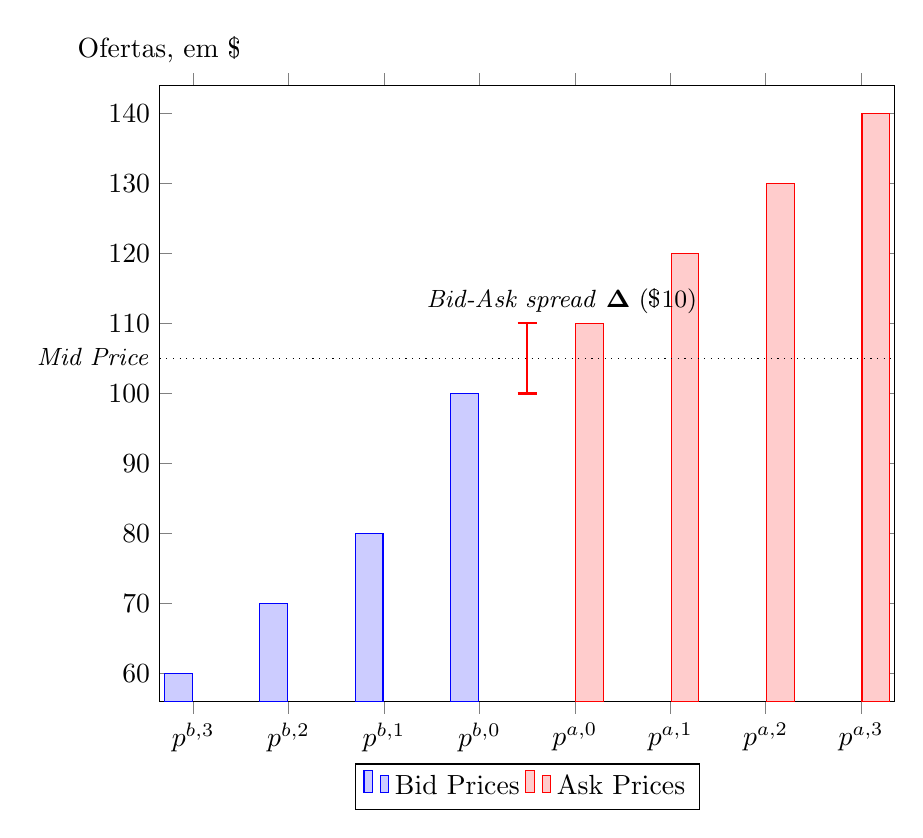
\begin{tikzpicture}
			\begin{axis}[
				x tick label style={/pgf/number format/1000 sep=},
				enlargelimits=0.05,
				legend style={at={(0.5,-0.1)}, anchor=north,legend columns=-1},
				ybar=0.7,
				ylabel={Ofertas, em \$},
    				ylabel style={
    				at={(0,1.02)},
    				anchor=south,
    				rotate=-90,
    			},
				width=0.9\textwidth, % Adjust the width to fit within the box
				xticklabels={
					$p^{b, 3}$, $p^{b, 2}$, $p^{b, 1}$, $p^{b, 0}$, 
					$p^{a, 0}$, $p^{a, 1}$, $p^{a, 2}$, $p^{a, 3}$
					},
				xtick={1,2,3,4,5,6,7,8}, % Set explicit tick positions
				after end axis/.code={
					\draw [red, thick, line cap=] (axis cs:4.5,100) -- (axis cs:4.5,110); % Static vertical line for spread with end caps
					\draw [red, thick] (axis cs:4.4,100) -- (axis cs:4.6,100);
					\draw [red, thick] (axis cs:4.4,110) -- (axis cs:4.6,110);
					\draw [black, dotted] (axis cs:0.65,105) -- (axis cs:8.35,105);
					\node[right, font=\small] at (rel axis cs:0.35,0.65) {\textit{Bid-Ask spread} $\mathbf{\Delta}$ (\$10)}; % Label for the spread line
					\node[left, font=\small] at (rel axis cs:0,0.56) {\textit{Mid Price}};
				}
				]
				% Represent bid prices in blue
				\addplot [blue, fill=blue!20] coordinates {(1, 60) (2, 70) (3, 80) (4, 100)};
				% Represent ask prices in red
				\addplot [red, fill=red!20] coordinates {(5, 110) (6, 120) (7, 130) (8, 140)};
				\legend{Bid Prices, Ask Prices}
			\end{axis}
		\end{tikzpicture}
	\end{center}
	\caption{Gráfico de ofertas de um livro de ordens limite $L$ qualquer}
\end{figure}

\begin{figure}[H]
	\begin{center}
		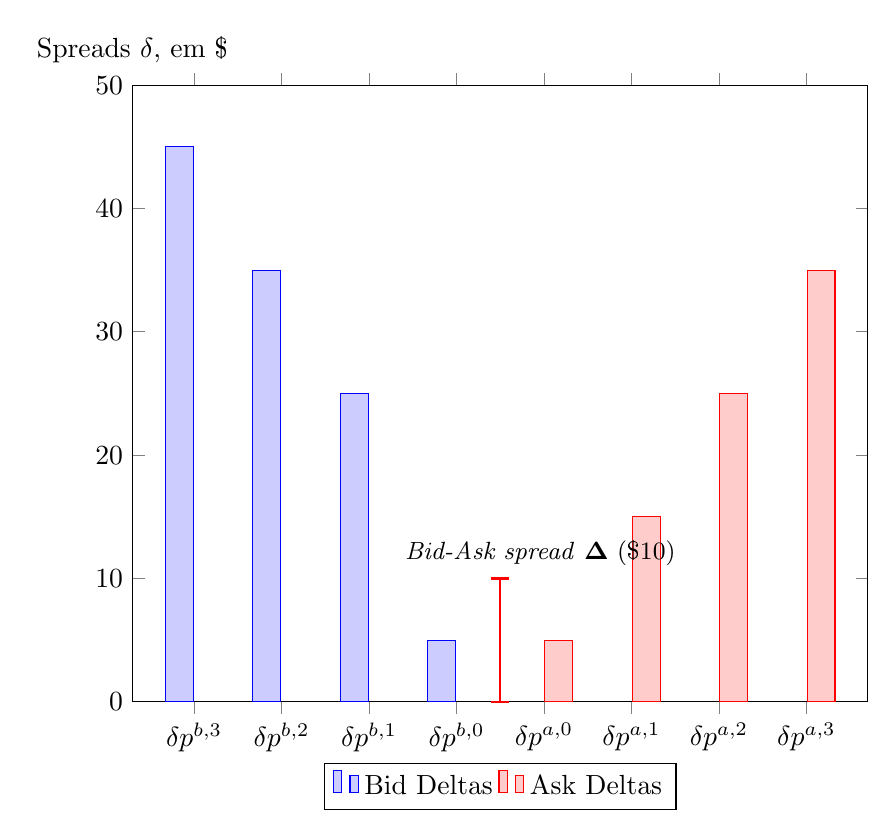
\begin{tikzpicture}
			\begin{axis}[
				x tick label style={/pgf/number format/1000 sep=},
				legend style={at={(0.5,-0.1)}, anchor=north,legend columns=-1},
				ybar=0.7,
				ylabel={Spreads $\delta$, em \$},
				ylabel style={
					at={(0,1.02)},
					anchor=south,
					rotate=-90,
				},
				ymin=0, ymax=50,
				width=0.9\textwidth, % Adjust the width to fit within the box
				xticklabels={
					$\delta p^{b, 3}$, $\delta p^{b, 2}$, $\delta p^{b, 1}$, $\delta p^{b, 0}$, 
					$\delta p^{a, 0}$, $\delta p^{a, 1}$, $\delta p^{a, 2}$, $\delta p^{a, 3}$
					},
				xtick={1,2,3,4,5,6,7,8}, % Set explicit tick positions
				after end axis/.code={
					\draw [red, thick, line cap=] (axis cs:4.5,0) -- (axis cs:4.5,10); 
					% Static vertical line for spread with end caps
					\draw [red, thick] (axis cs:4.4,0) -- (axis cs:4.6,0);
					\draw [red, thick] (axis cs:4.4,10) -- (axis cs:4.6,10);
					\node[right, font=\small] at (axis cs:3.3,12) {\textit{Bid-Ask spread} $\mathbf{\Delta}$ (\$10)}; % Label for the spread line
				}
				]
				% Represent bid prices in blue
				\addplot [blue, fill=blue!20] coordinates {(1, 45) (2, 35) (3, 25) (4, 5)};
				% Represent ask prices in red
				\addplot [red, fill=red!20] coordinates {(5, 5) (6, 15) (7, 25) (8, 35)};
				\legend{Bid Deltas, Ask Deltas}
			\end{axis}
		\end{tikzpicture}
	\end{center}
	\caption{Gráfico de spreads $\Delta$ de um livro de ordens limite $L$ qualquer}
\end{figure}

Para ilustrar melhor o funcionamento do livro de ordens considere a seguinte situação, para um único ativo: um agente qualquer de \textit{MM} tem a \textbf{única oferta de venda} pelo preço de $p^{(a, MM)}$ no mercado. Caso surja uma nova oferta de \textbf{compra} com melhor preço e acima do preço da oferta do agente $p^{(b, i)} \geq p^{(a, MM)}$, será gerada uma transação pelo preço $p^{(a, MM)}$ e a ordem de valor $p^{(b, i)}$ que gerou a transação é a ordem limite com preço de mercado. Após o motor de transações da bolsa receber a oferta $i$, uma transação ocorre e ambas ofertas são removidas do livro de ordens. 

O agente observa, para um determinado ativo e considerando novamente um índice de tempo discreto $t < T, t \in \mathbb{Z^{+}}$, três valores numéricos principais $(I_{t}, P_{t}, W_{t})$, sendo eles: 
\begin{itemize}
	\item o inventário $I_{t} \in \mathbb{Z}$ (a quantidade que têm do ativo);
	\item o preço médio do ativo $P_{t} \in \mathbb{R}$;
	\item o lucro financeiro do portfólio $W_{t} \in \mathbb{R}$;
	\item o valor total das negociações diárias, obtido a partir da expressão: $W_{t} + I_{t} \cdot P_{t}$;
\end{itemize}

A cada passo de tempo, ou seja, quando $t := t + 1$, o inventário do agente é atualizado da seguinte forma:
\begin{equation}
    \begin{aligned}
    	I_{t + 1} = N^{(b)}_{t + 1} - N^{(a)}_{t + 1} \label{eq:inventory}
    \end{aligned}
\end{equation}
onde $N^{(a)}$ e $N^{(b)}$ são as quantidades de ativos efetivamente vendidos ou comprados, distribuídas de acordo com um processo de contagem, com incrementos indepentes (note que os valores esperados dos incrementos dos processos seguem médias $\lambda_{t}^{(a)}$ e $\lambda_{t}^{(b)}$ que se alteram de acordo com o tempo $t$). Os incrementos dos processos de contagem são limitados externalmente à quantidade ofertada pelo agente, tal que $(N_{t + 1}^{(a)} - N_{t}^{(a)}) \leq Q_{t + 1}^{(a)}$ e $(N_{t + 1}^{(b)} - N_{t}^{(b)}) \leq Q_{t + 1}^{(b)}$.

O preço médio do ativo é facilmente obtido a partir de um movimento Browniano unidimensional (também chamado de processo de Wiener), de acordo com a equação incremental a seguir:
\begin{equation}
	\begin{aligned}
		P_{t+1} = P_t + \sigma \cdot \Delta Z_t
		\label{eq:midprice}
	\end{aligned}
\end{equation}
onde \(\sigma\) é a volatilidade do ativo e \(\Delta Z_t\) é uma variável aleatória amostrada de uma distribuição normal com média 0 e variância \(\Delta t\), onde \(\Delta t\) é o tamanho do intervalo de tempo discreto.

Por fim, o lucro financeiro do agente (também chamado de \textit{Profit and Loss} ou \textit{PnL}) é atualizado de acordo com a seguinte expressão:
\begin{equation}
	\begin{aligned}
		W_{t + 1} = W_{t} + p^{(a, MM)}_{t} \cdot (N^{(a)}_{t + 1} - N^{(a)}_{t}) - p^{(b, MM)}_{t} \cdot (N^{(b)}_{t + 1} - N^{(b)}_{t} )
		\label{eq:pnl}
	\end{aligned}
\end{equation}

A cada observação e atualização dos valores $(P_{t}, W_{t}, I_{t})$ o agente pode escolher não fazer nada ou realizar uma das ações abaixo:
\begin{enumerate}
    \item alterar as quantidades ofertadas $Q^{(a)}_{t + 1}$ e $Q^{(b)}_{t + 1}$;
    \item alterar os preços ofertados $p^{(a, MM)}_{t + 1}$ e $p^{(b, MM)}_{t + 1}$;
\end{enumerate}

O agente realiza essas mudanças buscando maximizar uma função-utilidade $U(X)$, que de preferência incorpore os valores do PnL, do inventário atual e do preço médio do ativo, assim como um fator de aversão ao risco. Para tal, definimos a progressão da recompensa $R$ em relação ao tempo $t$ como:

\begin{equation}
	\begin{aligned}
		R_{t + 1} = U(W_{t} + I_{t} \cdot P_{t})
		\label{eq:reward}
	\end{aligned}
\end{equation}

onde a função utilidade $U$ escolhida é exponencial, tal que $U(x) = -e^{-c x}$ e $c$ é o coeficiente de aversão ao risco.

Por fim, traduzindo os conceitos discutidos podem ser aplicado no contexto de aprendizado por reforço, formando o $MDP = (\mathcal{S}, \mathcal{A}, T_{a}, R_{a})$, onde o espaço de observações do ambiente é \(\mathcal{S} = \{(P, W, I) \mid P \in \mathbb{R}, W \in \mathbb{R}, I \in \mathbb{Z}\}\), o espaço de ações do agente é \(\mathcal{A} = \{(p^a, p^b, Q^a, Q^b) \mid p \in \mathbb{R}^+ \text{ e } Q \in \mathbb{N}\}\). Os valores do operador de transição $T$ são obtidos de acordo com as dinâmicas em \ref{eq:inventory}, \ref{eq:midprice} e \ref{eq:pnl} e os valores da função de recompensa é dada por \ref{eq:reward}.

\subsection{Técnicas possíveis e Metodologia escolhida para aproximar a solução da equação de Bellman}
\label{section:problem_description/techniques}
Em síntese, a otimização do retorno financeiro em operações de \textit{market-making} envolve desafios complexos, abordados por métodos analíticos tradicionais e soluções analíticas para tempo contínuo, mas que frequentemente enfrentam limitações na dinâmica do ambiente financeiro \citep{Avellaneda2008, rao2020stochastic, Gasperov2021}.

O aprendizado por reforço, notadamente com o algoritmo Soft Actor-Critic (SAC) e Deep Q-Learning (DQL), destaca-se pela sua adaptabilidade contínua às mudanças na dinâmica do sistema do mercado, oferecendo uma abordagem eficaz e flexível \citep{Ganesh2019, bakshaev2020marketmaking, Sutton2018}. A aplicação de técnicas como redes neurais de memória de curto prazo (LSTM) no aprendizado por reforço demonstra a capacidade de lidar com complexidades e padrões temporais nos mercados financeiros \citep{WOS:000747190900001}.

Embora as distintas abordagens apresentem vantagens e desvantagens, a escolha pelo aprendizado por reforço visa superar desafios e adaptar-se à complexidade computacional do ambiente \citep{WOS:000963297000001}. Assim, o uso do paradigma de aprendizado por reforço foi escolhido para obter a solução da equação de otimalidade de Bellman e da política do agente. Finalmente, a contribuição proposta nesta pesquisa consiste em integrar a aversão ao risco noturno à estratégia do agente, adicionando uma restrição que limita a exposição ao mercado no final do dia, ampliando assim a compreensão e gestão dos riscos associados ao \textit{market-making} \citep{almgren2000}. 

Existem algumas alternativas para formalizar matematicamente essa restrição:
\begin{enumerate}
    \item De forma simplificada, no final do dia o agente não pode ter nenhum ativo em posição: 
    \begin{equation}
        I_{T} = 0
        \label{eq:inventory_restriction}
    \end{equation}
    \item Com uma abordagem mais complexa, se houver alguma posição restante, o agente precisa \textit{headgear}\footnote{De maneira simplificada, o \textit{hedge} consiste em comprar ou vender ativos que tenham uma exposição ao risco oposta aos riscos da carteira atual, de modo a equilibrar a posição.} sua exposição ao risco ao participar em outros mercados abertos no momento, abordagem que chamamos de \textit{market making} \textbf{simultâneo}.
\end{enumerate}


\subsection{Inserção da restrição de risco \textit{overnight} e \textit{Market making} simultâneo}
\label{section:problem_description/multivariate_mm}
Ao considerarmos a situação em que o MM aplica a sua estratégia em diversos mercados simultaneamente observamos um aumento da complexidade, mas também das alternativas para lidar com riscos envolvidos - chamamos essa situação de MM \textbf{simultâneo} ou \textbf{multivariado}.

Para tal, consideramos a possibilidade do agente negociar um ativo $i$ dentre um total de $k$ ativos diferentes, em possivelmente diversos mercados. Os elementos do espaço de observações e de ações do agente passam a ser os vetores 
\[ 
\mathcal{S} = \{(\mathbf{P}, \mathbf{W}, \mathbf{I}) \mid \mathbf{P} \in \mathbb{R}^{k}, \mathbf{W} \in \mathbb{R}^{k}, \mathbf{I} \in \mathbb{Z}^{k}\}
\]
\[
\mathcal{A} = \left\{ (\mathbf{p}^a, \mathbf{p}^b, \mathbf{Q}^a, \mathbf{Q}^b) \mid \mathbf{p} \in \mathbb{R}^{k},  \mathbf{Q} \in \mathbb{N}^{k} \right\}
\].

O objetivo principal (\ref{eq:objective}) continua a mesmo, e remove-se a restrição (\ref{eq:inventory_restriction}). Contudo, surgem novas alternativas para proteção da carteira durante a noite:

\begin{enumerate}
    \item O agente pode avaliar o risco global da carteira, e incluir um único ativo de proteção contra o risco global ao final do dia.
    \item Se o ativo for negociado em múltiplas bolsas (chamado também de ativo \textit{co-listed}), o agente pode continuar a negociação deste em outra bolsa caso uma delas esteja fechada.
\end{enumerate}

Considerando um cenário em que haja ações em \textit{co-listing}, surge a possibilidade de criação de estratégias mais sofisticadas, permitindo a implementação dos itens mencionados acima.


\section{Trabalhos prévios}
\label{section:previous_works}
A pesquisa sobre a minimização de risco overnight usando Aprendizado por Reforço (RL) para estratégias de market making está inserida em um contexto mais amplo de estudos que exploram a aplicação do RL em finanças quantitativas. Nesta seção, levantamos uma lista inicial de trabalhos relacionados que ajudaram a moldar e fundamentar a proposta deste projeto.

A pesquisa formal do problema do \textit{Market Making} (MM) foi iniciada pelo estudo de  Marco Avellaneda e Sasha Stoikov, em seu trabalho seminal de 2008 \citep{Avellaneda2008}. Eles abordaram o problema do MM sob certas suposições relacionadas aos processos de chegada de ordens de compra e venda. No entanto, é importante observar que, nesse cenário, eles não impuseram a restrição de que o inventário do \textit{market maker} no final do dia fosse diferente de zero, ou seja, $q_T \neq 0$.

Como um dos resultados, Avellaneda e Stoikov conseguiram definir uma estratégia ótima para o MM, que se baseia em um cálculo cuidadoso das cotações de compra e venda em resposta às chegadas de ordens de mercado. Esta estratégia foi derivada dentro de um quadro teórico e matemático bem definido, oferecendo uma proposta clara sobre como um \textit{market maker} pode otimizar seu desempenho em um livro de ordens.

Ao longo do tempo, diversos autores começaram a relaxar algumas das hipóteses feitas por Avellaneda e Stoikov, tornando o cenário de MM mais genérico e realista. Esse avanço na literatura expandiu as possibilidades de modelagem e análise de estratégias de MM em ambientes mais complexos e dinâmicos. Alguns exemplos são:
\begin{itemize}
    \item ``Optimal Market Making with Limited Risk'' \citep{Gueant2017}: Este estudo aborda especificamente o problema do market making sob a perspectiva da minimização do risco. Os autores desenvolvem um modelo de market making que leva em consideração restrições de risco e investigam como otimizar a estratégia de market making enquanto limitam o risco associado.
    \item ``High-frequency trading in a limit order book'' \citep{Avellaneda2008}: Este estudo investiga as estratégias de trading de alta frequência em um livro de ordens de limite. Embora não aborde diretamente o uso do RL, fornece insights valiosos sobre o funcionamento de mercados eletrônicos e os desafios enfrentados pelos market makers, incluindo a gestão de risco e a necessidade de ajustar os preços rapidamente.
\end{itemize}


Nos últimos anos, o uso do paradigma de Aprendizado por Reforço se tornou mostrou extremamente útil para tarefas mais complexas, de jogos à medicina \citep{Kaelbling1996}. 
Aplicações específicas do método de \textit{RL} no estudo de problemas de \textit{MM} receberam grande atenção por alguns autores recentemente, notavelmente em:
\begin{itemize}
    \item "Reinforcement Learning Approaches to Optimal Market Making" \citep{Gasperov2021}: Este estudo fornece uma visão abrangente das aplicações do Aprendizado por Reforço em market making. Os autores demonstram como o RL pode ser usado para ajustar dinamicamente os preços de compra e venda em resposta às condições do mercado. Eles destacam a eficácia do RL em otimizar o retorno ajustado ao risco em comparação com estratégias tradicionais.
    \item "Reinforcement Learning for Market Making in a Multi-agent Dealer Market" \citep{Ganesh2019}: Este artigo oferece uma visão detalhada de como o RL pode ser aplicado em um ambiente de mercado com vários agentes, semelhante ao cenário do mundo real. Os autores demonstram que um agente de RL pode aprender a adaptar suas estratégias de market making em resposta às ações de outros agentes e às condições do mercado, incluindo a gestão de risco.
\end{itemize}


Ao revisar esses trabalhos relacionados, podemos observar que, apesar dos tratamentos teóricos bem elaborados, a situação real do uso do MM não se encaixa nas limitações impostas pelas pesquisa:

\begin{itemize}
    \item nos mercados financeiros reais, os agentes operam de uma forma mais complexa que assumido nas pesquisas: quase todos usam estratégias MM simultâneas;
    \item as alternativas de proteção e as restrições de posicionamento, especialmente numa estratégia simultânea, são bem mais abrangentes que na literatura atual. 
\end{itemize}

Em situações reais, diferente da proposta de \citet{Avellaneda2008}, não é possível encontrar uma estratégia ótima de forma analítica. O uso de técnicas de Aprendizado por Reforço em estratégias de market making oferece um potencial significativo para melhorar a eficiência das operações financeiras e mitigar os riscos associados, especialmente o risco overnight. 



\section{Objetivos}
\label{section:objectives}
A pesquisa tem como objetivo central a criação de uma estratégia específica de \textit{market making} ótima. Nesse contexto, planejamos obter tanto um método para otimização da política de escolha de preços, como também da criação do ambiente de simulação para o livro de ofertas limite e de outros agentes participantes do mercado.

O foco principal é a aplicação de técnicas de aprendizado por reforço para modelar o comportamento do agente de market making e inserir uma restrição essencial para minimizar o risco do agente. Em cenários onde a calibragem de parâmetros é necessária, serão realizados ajustes dos mesmos ao longo do tempo, de modo a levar em consideração as condições do mercado e as expectativas do agente.

Como conclusão da pesquisa, pretendemos realizar uma avaliação abrangente do desempenho da estratégia de market making, incluindo mas não limitado a análise do retorno da carteira ao longo do tempo, levando em consideração custos de transação e flutuações nos preços dos ativos. Avaliaremos também a eficácia da estratégia sob a restrição de risco \textit{overnight} máximo e o impacto das ordens geradas para zerar a carteira na liquidez do mercado. Após o treinamento do agente, realizaremos também uma análise comparativa entre a estratégia desenvolvida e estratégias tradicionais de mercado, especificamente de \textit{price-taking}. Isso nos permitirá destacar as vantagens e desvantagens da abordagem de aprendizado de reforço e comparar estatisticamente os resultados obtidos.


\section{Metodologia}
\label{section:methodology}
\section{Methodology}

\subsection{Problem Definition}
The market-making problem addressed in this work involves designing an optimal trading policy for an agent using reinforcement learning (RL). The agent aims to maximize profit while managing risks, particularly inventory risk. The market dynamics are modeled by the limit order book (LOB) and its dynamics, which define how the book evolves over time based on order flow and price movements. Our agent interacts with this environment by quoting bid and ask prices and adjusting offered quantities. As discussed previously, the main challenge for choosing an adequate agent and its policy lies in balancing profitability with risk management, especially regarding inventory at the close of the market, where overnight positions can expose the agent to significant risks.

\subsection{Formal Description of the RL Environment} In modeling the RL environment, we initially utilize a continuous-time, continuous-state Markov Chain framework, and later transition to a discrete representation to address computational space constraints. We choose a state space that tries to best incorporate the historical events of the limit order book into a single observable state using commonly used indicators and LOB levels, as well as intrinsic features to the agent as proposed by <multiple references, inserir paper com review de RL para MM>. Given our performed bibliographical research, we chose the agent's current inventory for the intrinsic feature and a set of indicators for the extrinsic features: the Relative Strength Index (RSI); order imbalance (O); and micro price (MP). Additionally, for a fixed number $D$ of LOB price levels the pair $(\delta^d, Q^d)$, where $\delta^d$ is the half-spread distance for the level $d \leq D$, and $Q^d$ the amount of orders posted at that level is added to the state as a set of tuples, for both the ask and bid sides of the book. The state space can therefore be formally expressed as:
$$
X_t = (I_t, \, RSI_t, \, O_t, \, \text{MP}_t, \, \{ (\delta_t^{d, \text{ask}}, Q_t^{d, \text{ask}}) \}_{d=1}^D, \, \{ (\delta_t^{d, \text{bid}}, Q_t^{d, \text{bid}}) \}_{d=1}^D)
$$
As mentioned, the evolution is continuous in time, meaning state changes occur at any point in continuous time, and the next event occurs after a sampled waiting time. The specific case in which a Markov Chain also has an associated reward distribution $R$ for each state transition is called a Markov Reward Process and given that the MM problem also has a decision process that affects the transition probabilities it is therefore called a Markov Decision Process in control literature, and is generically defined as a 4-tuple $ (\mathcal{S}, \mathcal{A}, \mathbb{P}, R) $, where:

\begin{itemize}
	\item $\mathcal{S}$ is a set of states called the state space.
	\item $\mathcal{A}$ is a set of actions called the action space.
	\item $P: \mathcal{S} \times \mathcal{A} \times \mathcal{S} \to [0, 1]$ is the transition probability function for the MDP.
	\item $R: \mathcal{S} \times \mathcal{A} \times \mathcal{S}' \rightarrow \mathbb{R}$ is the reward function associated with each state transition.
\end{itemize}

Furthermore, the decision process will be defined in detail, as well as its effects on the choice of actions and the transition probability.

\subsection{State Transition Distribution and Environment Evolution Dynamics}

The previously mentioned transition probability density $P$ is given by a Stochastic Differential Equation expressed by the Kolmogorov forward equation for Markov Decission Processes:

\begin{equation}
	\frac{\partial P(s', t | s, a)}{\partial t}  = \int_{\mathcal{S}} \mathcal{L}(s' | a, t) P(x| s, a, t) dx
\end{equation}

for all $s, s' \in \mathcal{S}$ and all times $t$ before market end $T$, that is, $t \le T$, where $a$ is choosen by our control agent according to a policy $\pi (s)$. $\mathcal{L}$ is the generator operator and governs the dynamics of the state transitions given the current time. It's expression is obtained by deriving the closed-form expression for the dynamics of the underlying model, and for simple models such as those proposed by <avellaneda & stoikov, gueant>, the closed-form expression has been calculated. The underlying model for this paper is more complex, and solving for the respective generator operator is outside the scope of this paper, and a numerical approximation will be used furthermore when we define the models for the Proximal Policy Optimization (PPO) and Advantage Actor Critic (A2C) in Section 5 <inserir link>.

\subsubsection{Chosen State Space}
In continuous-time and continuous-state MDPs, the state $S$ evolves as a continuous-time stochastic process with dynamics reflected by $\mathcal{L}$ and - as mentioned - modern approaches to Reinforcement Learning require solving either numerically or approximating its transition probabilities. For our choosen market simulation model, we first formally define each component of our proposed state space:

\begin{itemize}
	$$
	\mathbf{S}_t = \left( \text{RSI}_t, \text{OI}_t, P_{\text{micro},t}, \Delta P_{1,t}, \Delta P_{2,t}, \dots, \Delta P_{d,t} \right) \in \mathbb{R}^3 \times \mathbb{R}^{2d}.
	$$
	
	The components of the state space are defined as follows:
	
	- \textbf{Order Imbalance (OI):} Order imbalance measures the relative difference between buy and sell orders at a given time. It is defined as:
	$$
	\text{OI}_t = \frac{Q_t^{\text{bid}} - Q_t^{\text{ask}}}{Q_t^{\text{bid}} + Q_t^{\text{ask}}},
	$$
	where \( Q_t^{\text{bid}} \) and \( Q_t^{\text{ask}} \) represent the total bid and ask quantities at time \( t \), respectively. \( \text{OI}_t \in [-1, 1] \), with \( \text{OI}_t = 1 \) indicating complete dominance of bid orders, and \( \text{OI}_t = -1 \) indicating ask order dominance.
	
	- \textbf{Relative Strength Index (RSI):} The RSI is a momentum indicator that compares the magnitude of recent gains to recent losses to evaluate overbought or oversold conditions. It is given by:
	$$
	\text{RSI}_t = 100 - \frac{100}{1 + \frac{\text{Average Gain}}{\text{Average Loss}}},
	$$
	where the \textit{Average Gain} and \textit{Average Loss} are computed over a rolling window (commonly 14 periods). Gains are the price increases during that window, while losses are the price decreases.

	- \textbf{Micro Price (\( P_{\text{micro}} \)):} The micro price is a weighted average of the best bid and ask prices, weighted by their respective quantities:
	$$
	P_{\text{micro},t} = \frac{P_t^{\text{ask}} Q_t^{\text{bid}} + P_t^{\text{bid}} Q_t^{\text{ask}}}{Q_t^{\text{bid}} + Q_t^{\text{ask}}},
	$$
	where \( P_t^{\text{ask}} \) and \( P_t^{\text{bid}} \) represent the best ask and bid prices at time \( t \).
	$$
\end{itemize}

\subsubsection{Chosen Action Space}

The control, or agent, interacts with the environment choosing actions from the set of possible actions, such that $a \in \mathbf{A}$ in response to observed states $s \in \mathbf{S}$ according to a policy $\pi (s, a)$ which we define shortly, and the goal is to maximize cumulative rewards over time. The system's dynamics depend on the agent's chosen action, so as to introduce features of market impact into our model, and the transition probabilities between states therefore depend on the agent's actions.

The action space $\mathcal{A}_t$ includes the decisions made by the agent at time $t$, specifically the desired bid and ask spreads pair $\delta_t^{\text{ask}}, \delta_t^{\text{bid}}$ and the corresponding posted order quantities $Q_t^{\text{ask}}, Q_t^{\text{bid}}$. Formally:
$$
\mathbf{A}_t = \left( \delta_t^{\text{ask}}, \delta_t^{\text{bid}}, q_t^{\text{ask}}, q_t^{\text{bid}} \right) \in \mathbb{R}^2 \times \mathbb{Z}^2.
$$

\subsubsection{Episodic Reward Function and Returns}

The episode reward function $r_t \in \mathbb{R}$ reflects the agent's profit and inventory risk obtained during a specific time in a past episode, it's value is given by the immediate reward function $R$, and differently from the instantaneous reward function it is discrete in time, so as to match observed event times (order arrivals and transactions occured). It depends on the spread and executed quantities, as well as the inventory cost and was choosen according to commonly used reward structures taken from the literature review.

The overall objective is to maximize cumulative utility while minimizing risk associated with inventory positions, and later insert restrictions so the risk for inventory is either limited at zero at market close, or incurring in larger penalties on the received rewards. For our model the utility chosen is based on a running Profit and Loss (PnL) score while still managing inventory risk. The choosen reward function is based on a risk-aversion enforced utility function, specifically the \textit{constant absolute risk aversion (CARA)}:

The PnL at time $t$ is computed as:
$$
\text{PnL}_t = \delta_t^{\text{ask}} q_t^{\text{ask}} - \delta_t^{\text{bid}} q_t^{\text{bid}} + \text{I}_t \cdot \Delta M_t.
$$

The agent starting penalty for holding large inventory positions  is discounted from the \textit{PnL} score, as follows:
$$
\text{Penalty}_t = \eta \left( \text{Inventory}_t \cdot \Delta M_t \right)^+,
$$
$$
\text{PnL}_t := \text{PnL}_t - \text{Penalty}_t
$$
where \( \eta \) is the penalty factor applied to positive inventory changes.

$$
R_t = U(\text{PnL}_t) = -e^{-\gamma \cdot \text{PnL}_t},
$$
where \( \gamma \) is the risk aversion parameter.

<inserir explicacao do para que serve o return>

\begin{equation}
G(\tau) = \int_0^T e^{-\gamma t} R(s_{t+dt}, s_t, a_t) \, dt
\end{equation}

\subsection{Model Description and Environment Dynamics}

For our model of the limit order book the timing of events follows a \textit{Hawkes process} so as to represent a continuous-time MDP that captures the usual observed pattern of clustered order arrival times.

The Hawkes process is a \textit{self-exciting process}, where the intensity \( \lambda(t) \) depends on past events. Formally, the intensity \( \lambda(t) \) evolves as:
$$
\lambda(t) = \mu + \sum_{t_i < t} \phi(t - t_i),
$$
where \( \mu > 0 \) is the baseline intensity, and \( \phi(t - t_i) \) is the \textit{kernel function} that governs the decay of influence from past events \( t_i \). A common choice for \( \phi \) is an exponential decay:
$$
\phi(t - t_i) = \alpha e^{-\beta (t - t_i)},
$$
where \( \alpha \) controls the magnitude of the self-excitation and \( \beta \) controls the rate of decay.

The bid and ask prices for each new order are modeled by two separate \textit{Ornstein-Uhlenbeck (OU) processes} to capture the mean-reversion behavior of spreads over the midprice:
$$
ds_t = \theta(\mu - s_t) dt + \sigma dW_t,
$$
where \( s_t \) is the market spread at time \( t \), \( \theta \) is the rate of mean reversion, \( \mu_{spread} \) is the long-term spread mean and \( \sigma \) its volatility. The Wiener process \( W_t \) is used to represent random market fluctuations.

The bid and ask spreads \( \delta_t^{\text{bid}} \) and \( \delta_t^{\text{ask}} \) for orders conditioned on their arrival follow normal distributions:
$$
\delta_t^{\text{ask}} \sim \mathcal{N}(\mu + M_{t-1} + s_t, \sigma^2), \quad a_t^{\text{bid}} \sim \mathcal{N}(\mu + M_{t-1} - s_t, \sigma^2),
$$
where \( \mu_{\text{ask}} \) and \( \mu_{\text{bid}} \) are the respective means and \( \Delta a_t \) is the spread adjustment. Whenever a new limit order that narrows the bid-ask spread or a market order arrive the mid-price is updated to reflect the top-of-book orders. The mid-price \( M \) at time $t+1$ is then obtained by averaging the maximum and minimum bid and ask prices in the book:

$$
M_{t+1} = \frac{2M_t + \delta^{ask}_{t} - \delta^{bid}_{t}}{2} 
\sim \mathcal{N}(\mu + M_{t}, \frac{\sigma^2}{2})
$$ and at $t = 0$, the midprice is defined according to some starting point of the model, usually an observed historical price as is chosen for our simulation as well.

The average of the top of book bid and ask prices therefore evolves according to a \textit{Brownian Motion} process:
$$
dM_t = \mu dt + \frac{\sigma^2}{2} dW_t,
$$
where \( W_t \) is a Wiener process and since the midprice is given by the sum of the top of book ask and bid prices, orders that cross the spread are usually rare and reflect a common stylized fact of LOBs in the market <inserir referencia book HFT>.

The order quantities \( q_t^{\text{ask}} \) and \( q_t^{\text{bid}} \) are modeled as Poisson random variables:
$$
q_t^{\text{ask}}, q_t^{\text{bid}} \sim \text{Poisson}(\lambda_q),
$$
where \( \lambda_q \) is the average order size.

\subsection{Decision Process and Steps to Maximize the Agent's Objective}

To express the Bellman equation for continuous-time MDPs, we consider the value function $V(s', a, s), which represents the expected total reward from state \( X \) under the optimal policy \( \pi^* \). The Bellman equation for a continuous-time MDP is:

<nao sei o que nao sei o que la> - pegar da proposta II enviada à FAPESP.



\bibliographystyle{apalike}
\renewcommand{\refname}{Referências}
\bibliography{reinforcement_learning.bib}

\end{document}